\chapter{IPv6: Part 1}\label{ipv6-part-1}

HEXIDECIMAL (Review)

\begin{figure}
\centering
\pandocbounded{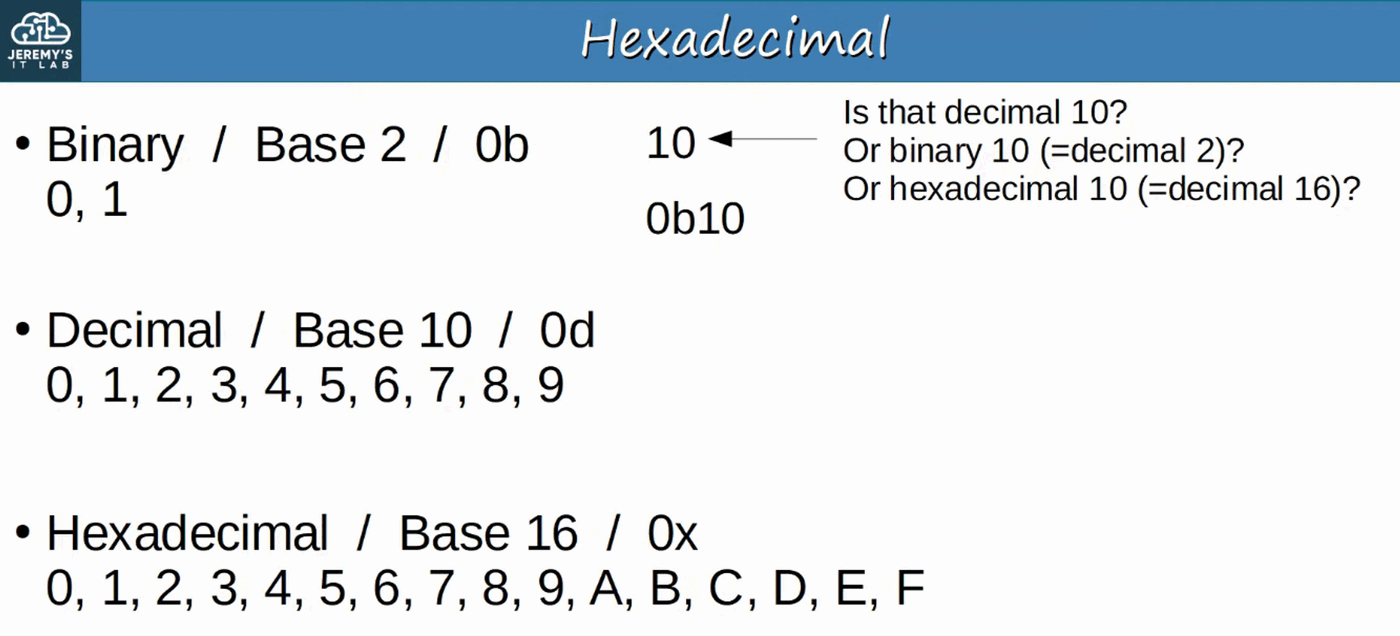
\includegraphics[keepaspectratio,alt={image}]{images/32-ipv6-part1/img-001.png}}
\end{figure}

\begin{figure}
\centering
\pandocbounded{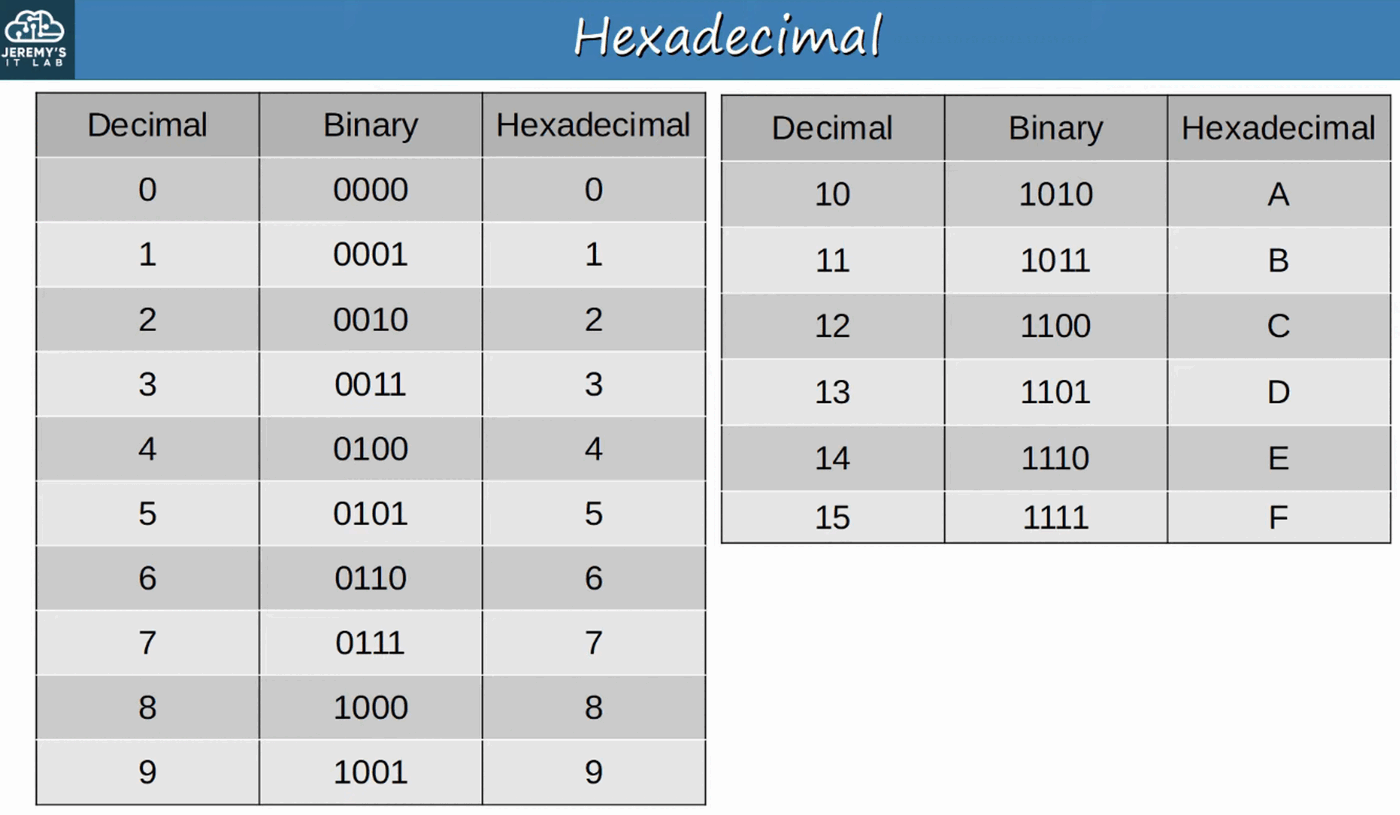
\includegraphics[keepaspectratio,alt={image}]{images/32-ipv6-part1/img-002.png}}
\end{figure}

\begin{figure}
\centering
\pandocbounded{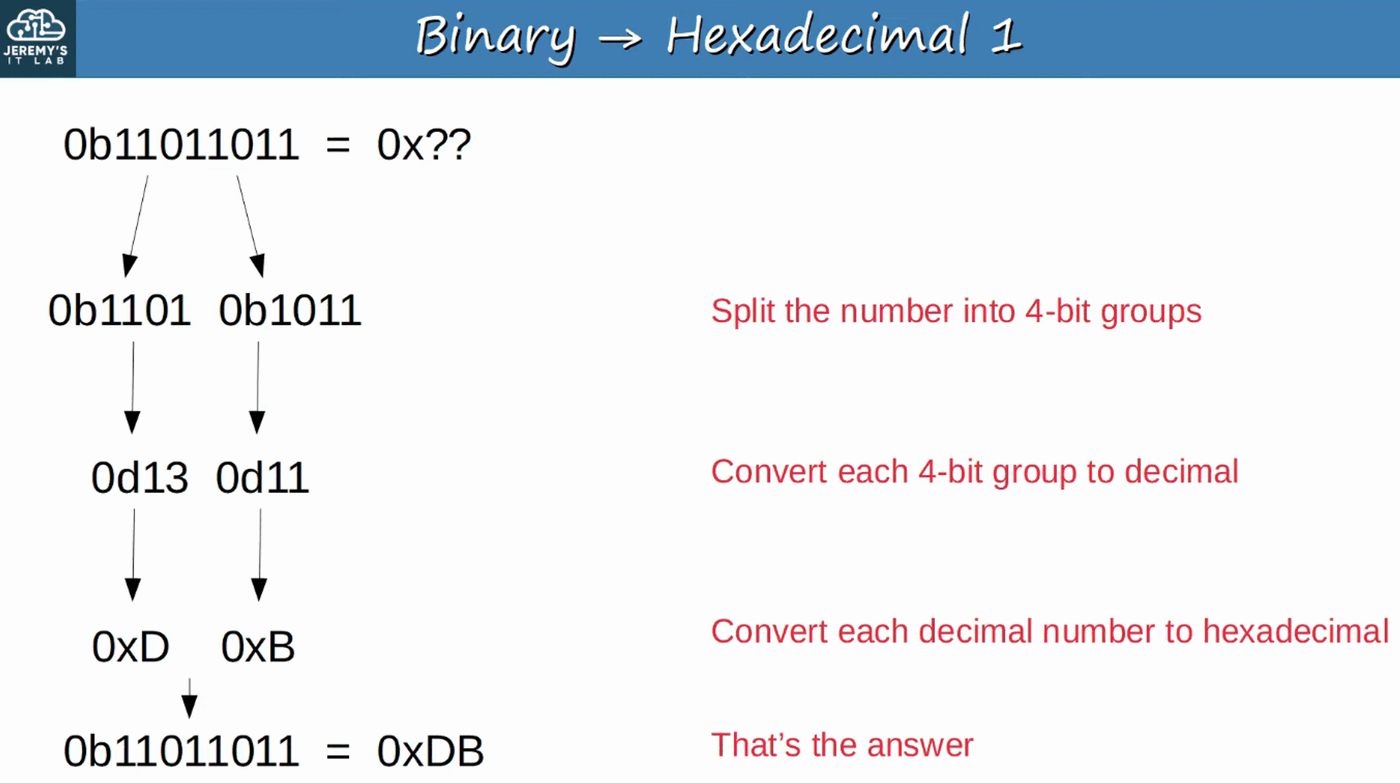
\includegraphics[keepaspectratio,alt={image}]{images/32-ipv6-part1/img-003.png}}
\end{figure}

What about the reverse (Hex to Binary) ???

\begin{figure}
\centering
\pandocbounded{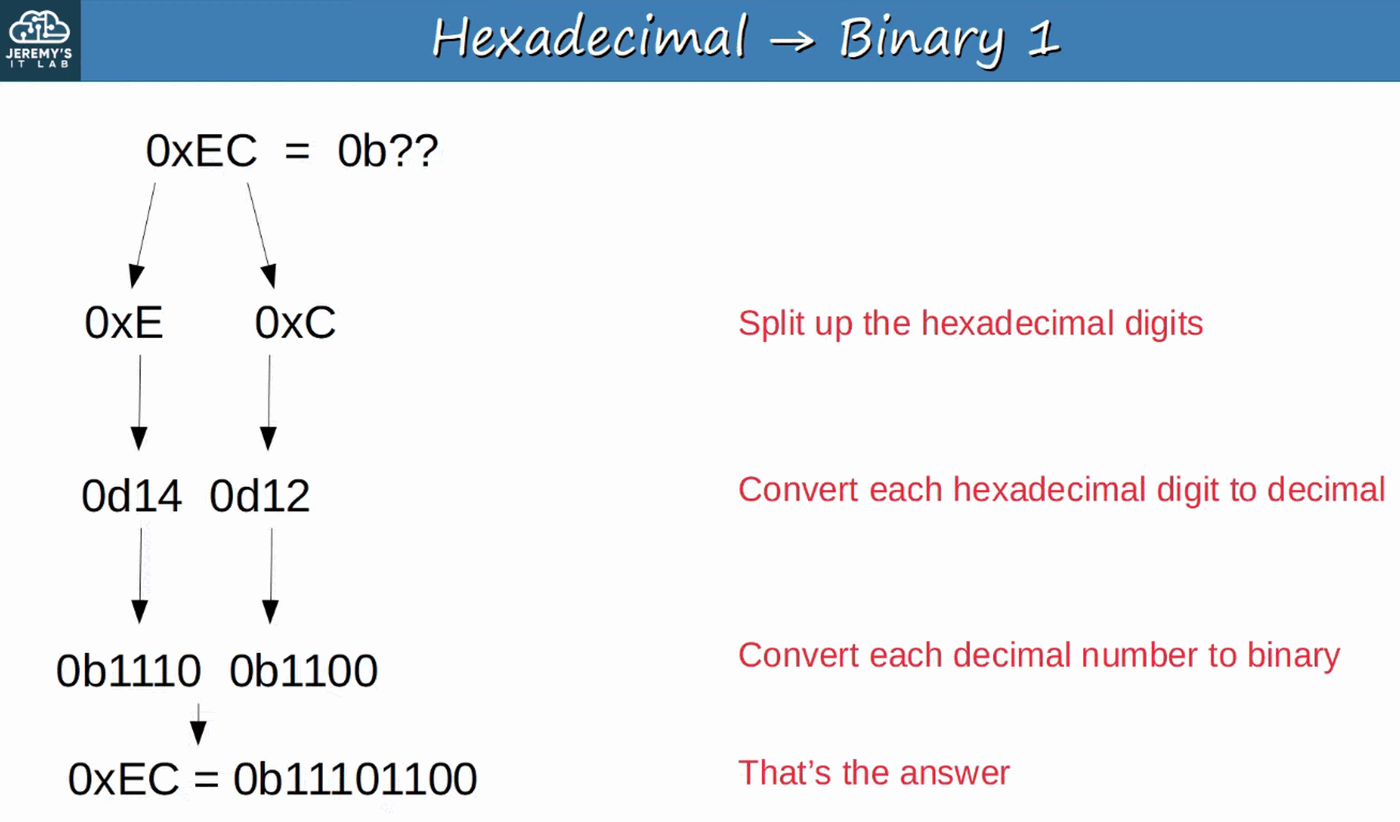
\includegraphics[keepaspectratio,alt={image}]{images/32-ipv6-part1/img-004.png}}
\end{figure}

WHY IPv6?

\begin{itemize}
\item
  The \textbf{MAIN REASON} is that there are simply not enough IPv4
  addresses available
\item
  There are 2\^{}32 IPv4 Addresses available (4,294,967,296)
\item
  When IPv4 was being designed 30 years ago, the creators had NO idea
  the Internet would be as large as today
\item
  VLSM, Private IPv4 ADDRESSES, and NAT have been used to conserve the
  use of IPv4 ADDRESS SPACE.

  \begin{itemize}
  \tightlist
  \item
    These are short-term solutions, however.
  \end{itemize}
\item
  The LONG -TERM solution is IPv6
\item
  IPv4 ADDRESS assignments are controlled by IANA (Internet Assigned
  Number Authority)
\item
  IANA distributes IPv4 ADDRESS space to various RIRs (Regional Internet
  Registries), which then assign them to companies that need them.
\end{itemize}

\begin{figure}
\centering
\pandocbounded{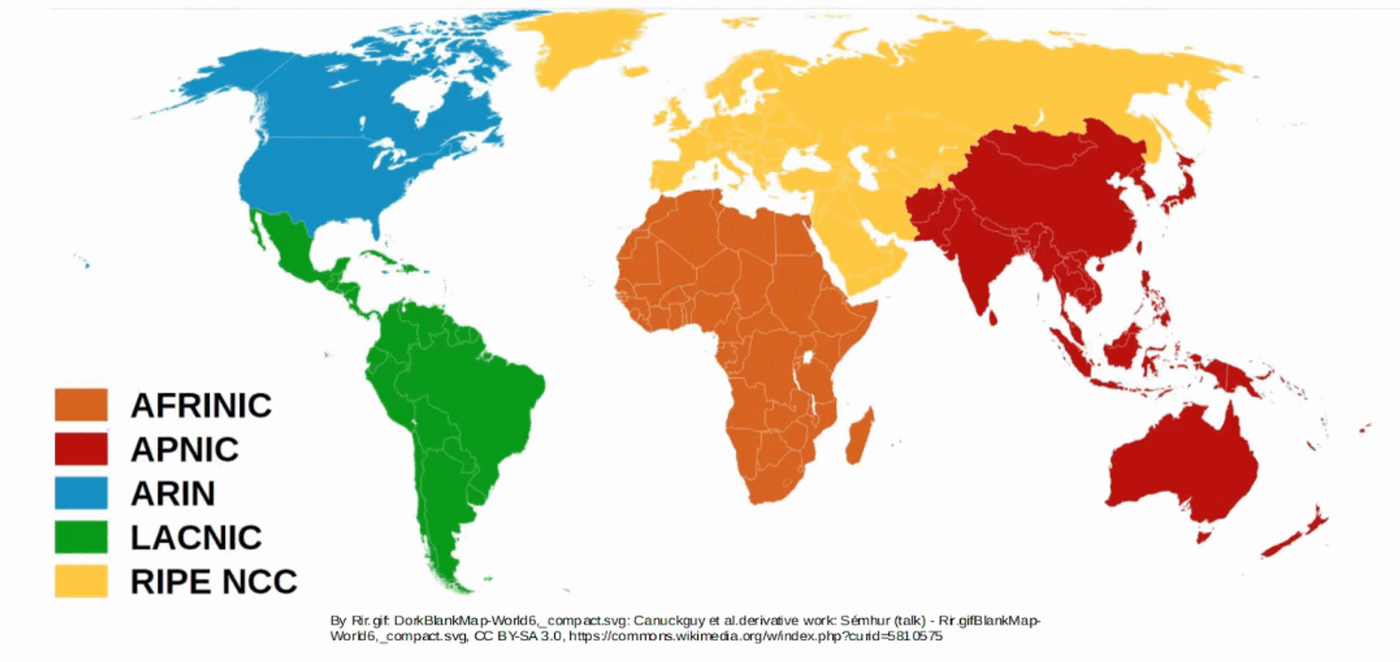
\includegraphics[keepaspectratio,alt={image}]{images/32-ipv6-part1/img-005.png}}
\end{figure}

\begin{itemize}
\tightlist
\item
  On September 24th, 2015, ARIN declared exhaustion of the ARIN IPv4
  address pool
\item
  On August 21st, 2020, LACNIC announced that it had made its final IPv4
  allocation
\end{itemize}

BASICS OF IPv6

\begin{itemize}
\tightlist
\item
  An IPv6 ADDRESS is \textbf{128 bits (8 ``groups'', 16 bits per
  ``group''. Groups are separated by `:')}
\end{itemize}

\begin{figure}
\centering
\pandocbounded{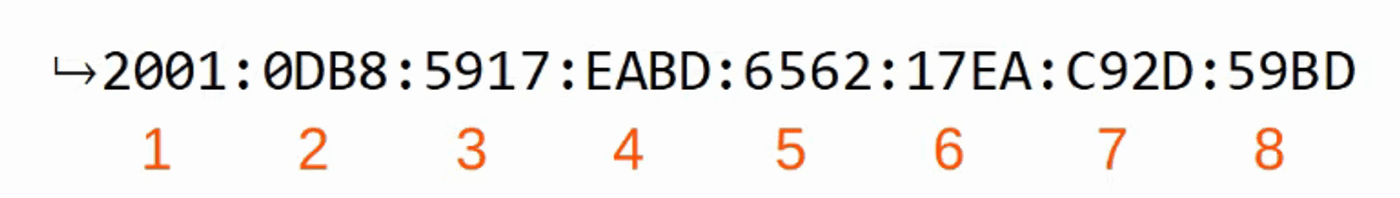
\includegraphics[keepaspectratio,alt={image}]{images/32-ipv6-part1/img-006.png}}
\end{figure}

\begin{itemize}
\tightlist
\item
  An IPv6 ADDRESS uses the / prefix number
\end{itemize}

SHORTENING (Abbreviating) IPv6 ADDRESSES

\begin{figure}
\centering
\pandocbounded{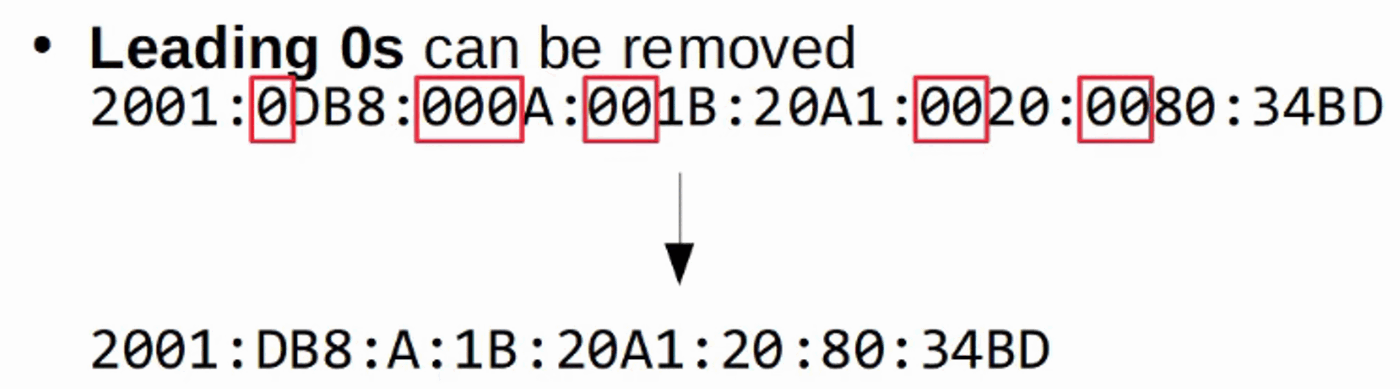
\includegraphics[keepaspectratio,alt={image}]{images/32-ipv6-part1/img-007.png}}
\end{figure}

\begin{figure}
\centering
\pandocbounded{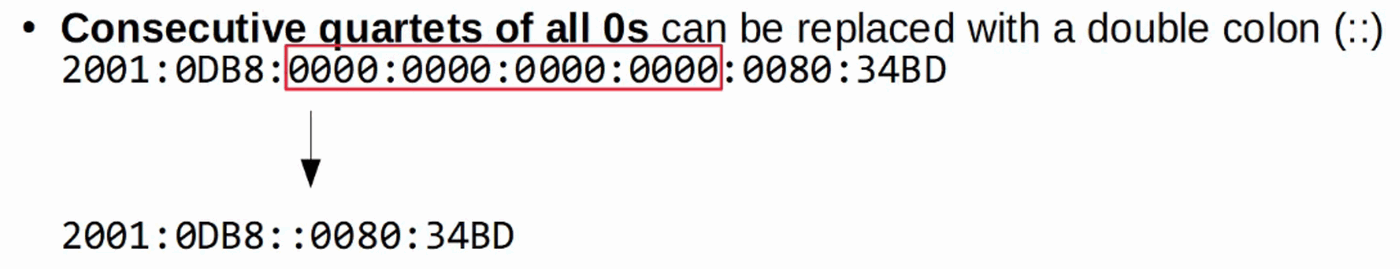
\includegraphics[keepaspectratio,alt={image}]{images/32-ipv6-part1/img-008.png}}
\end{figure}

\begin{figure}
\centering
\pandocbounded{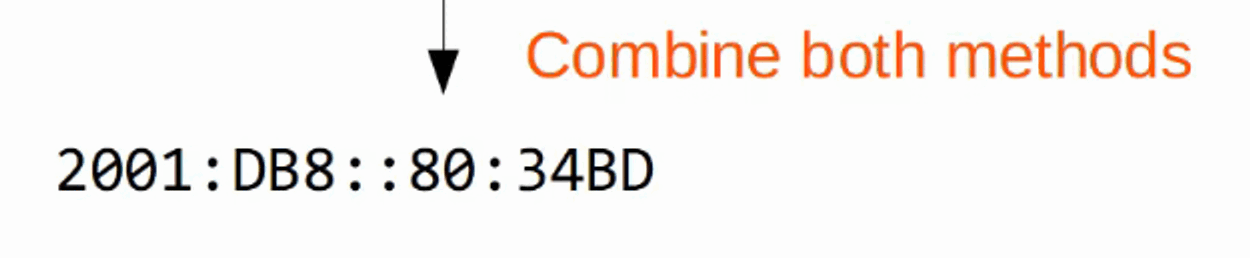
\includegraphics[keepaspectratio,alt={image}]{images/32-ipv6-part1/img-009.png}}
\end{figure}

\begin{figure}
\centering
\pandocbounded{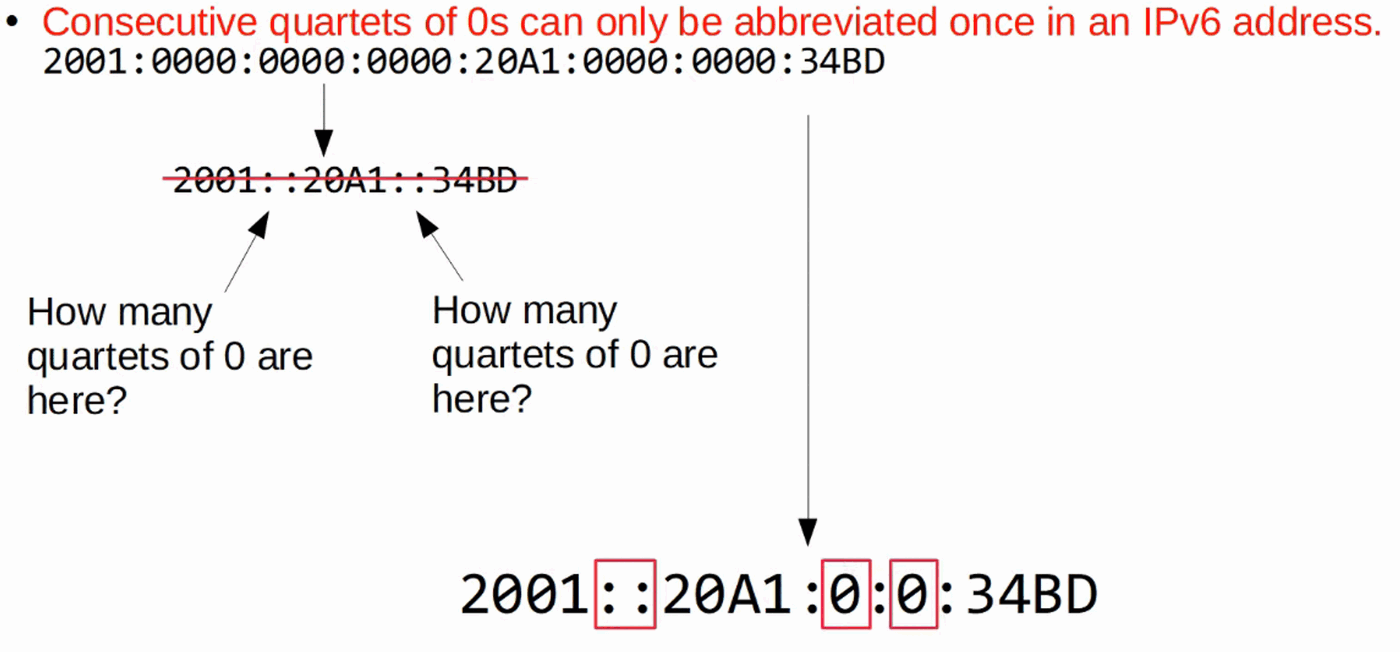
\includegraphics[keepaspectratio,alt={image}]{images/32-ipv6-part1/img-010.png}}
\end{figure}

\begin{figure}
\centering
\pandocbounded{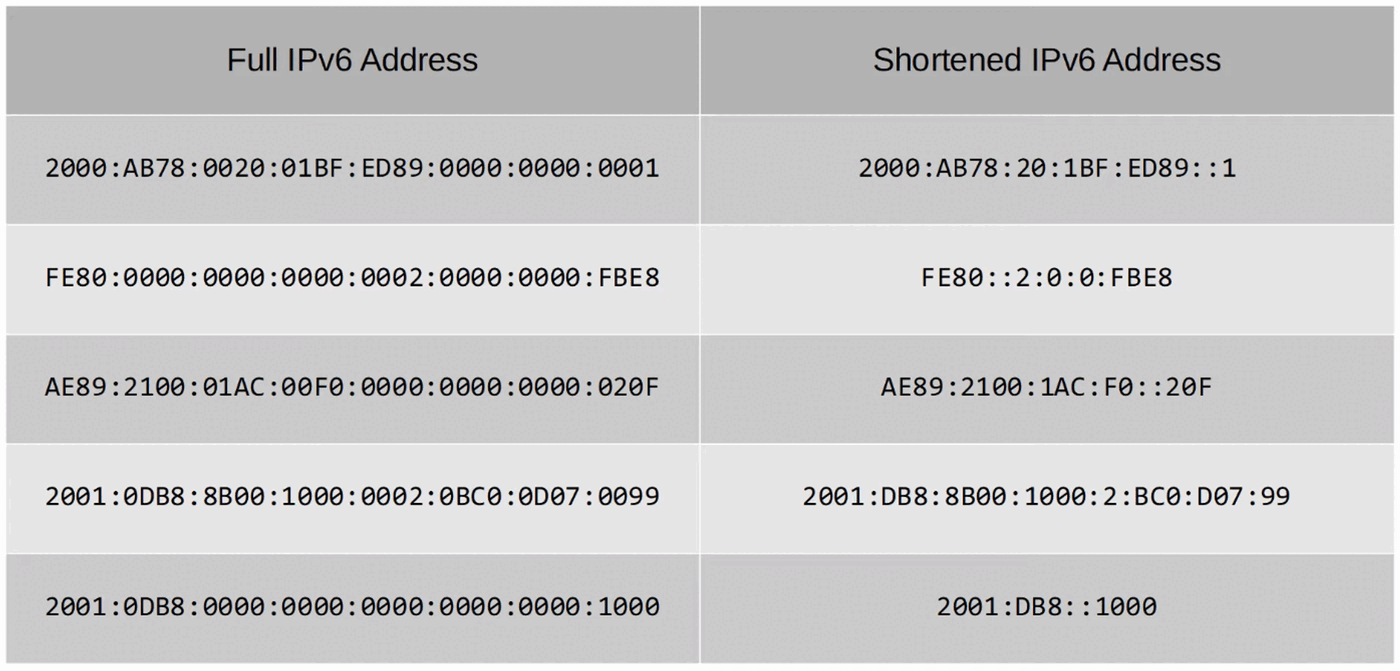
\includegraphics[keepaspectratio,alt={image}]{images/32-ipv6-part1/img-011.png}}
\end{figure}

EXPANDING (Abbreviating) IPv6 ADDRESSES

\begin{figure}
\centering
\pandocbounded{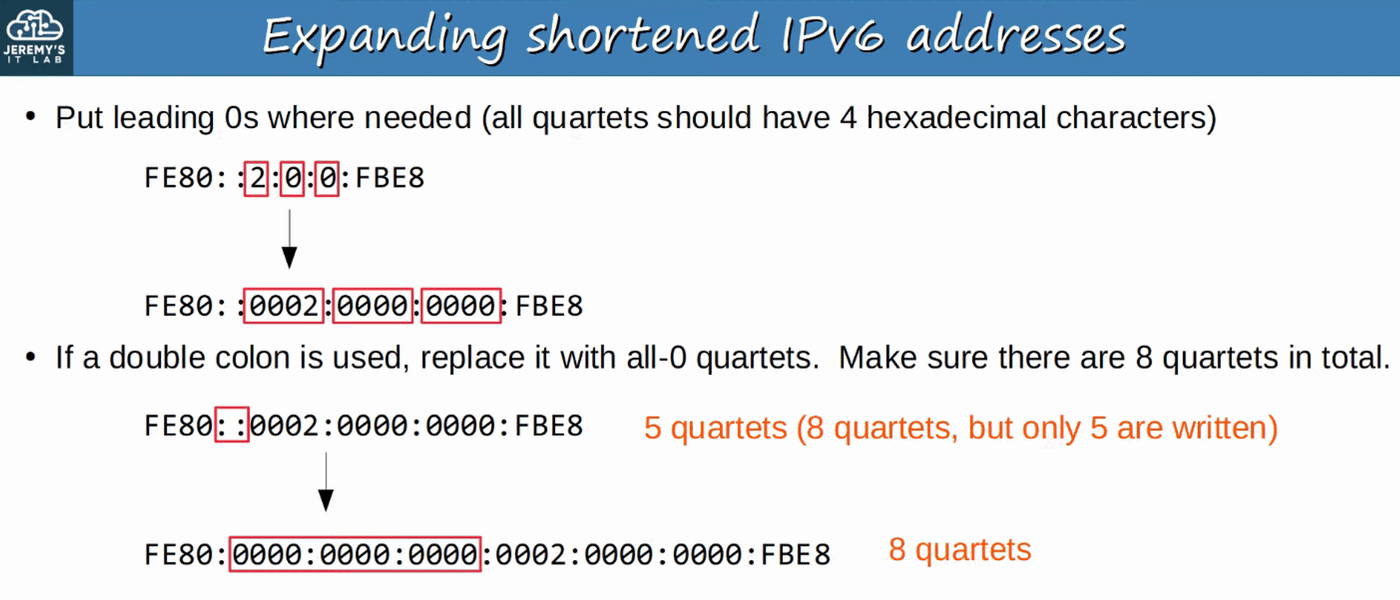
\includegraphics[keepaspectratio,alt={image}]{images/32-ipv6-part1/img-012.png}}
\end{figure}

FINDING the IPv6 PREFIX (GLOBAL UNICAST ADDRESSES)

\begin{itemize}
\tightlist
\item
  Typically, an Enterprise requesting IPv6 ADDRESSES from their ISP will
  receive a /48 BLOCK
\item
  Typically, IPv6 SUBNETS use a /64 PREFIX LENGTH
\item
  That means an Enterprise has 16 bits to use to make SUBNETS
\item
  The remaining 64 bits can be used for HOSTS
\end{itemize}

\begin{figure}
\centering
\pandocbounded{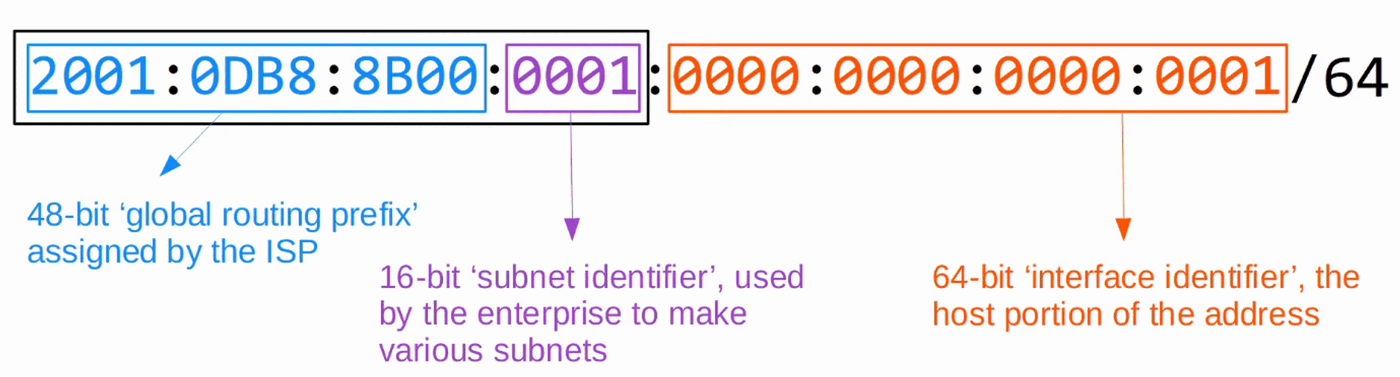
\includegraphics[keepaspectratio,alt={image}]{images/32-ipv6-part1/img-013.png}}
\end{figure}

\begin{figure}
\centering
\pandocbounded{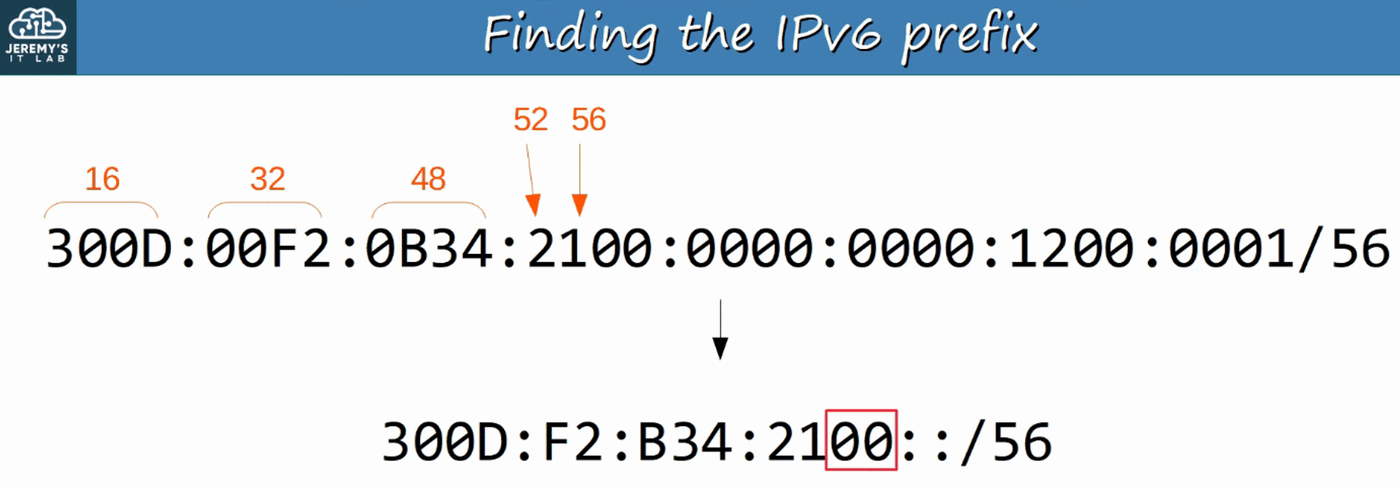
\includegraphics[keepaspectratio,alt={image}]{images/32-ipv6-part1/img-014.png}}
\end{figure}

(Each digit is 4 bits / each 4 digit block is 16 bits)

\textbf{REMEMBER} : You can only remove the LEADING ZEROS !!!

2001 : 0DB8 : 8B00 : 0001 : FB89 : 017B : 0020 : 0011 /93

Because 93 lands in the middle of a 4 bit number, we need to convert the
last digit to binary and borrow a ``bit'' from the first binary digit.

:: 017 {[}B{]} :: B = 0d11 = 0b1011 = 0b1000 (the first digit is
borrowed, the remainder become 0)

\begin{figure}
\centering
\pandocbounded{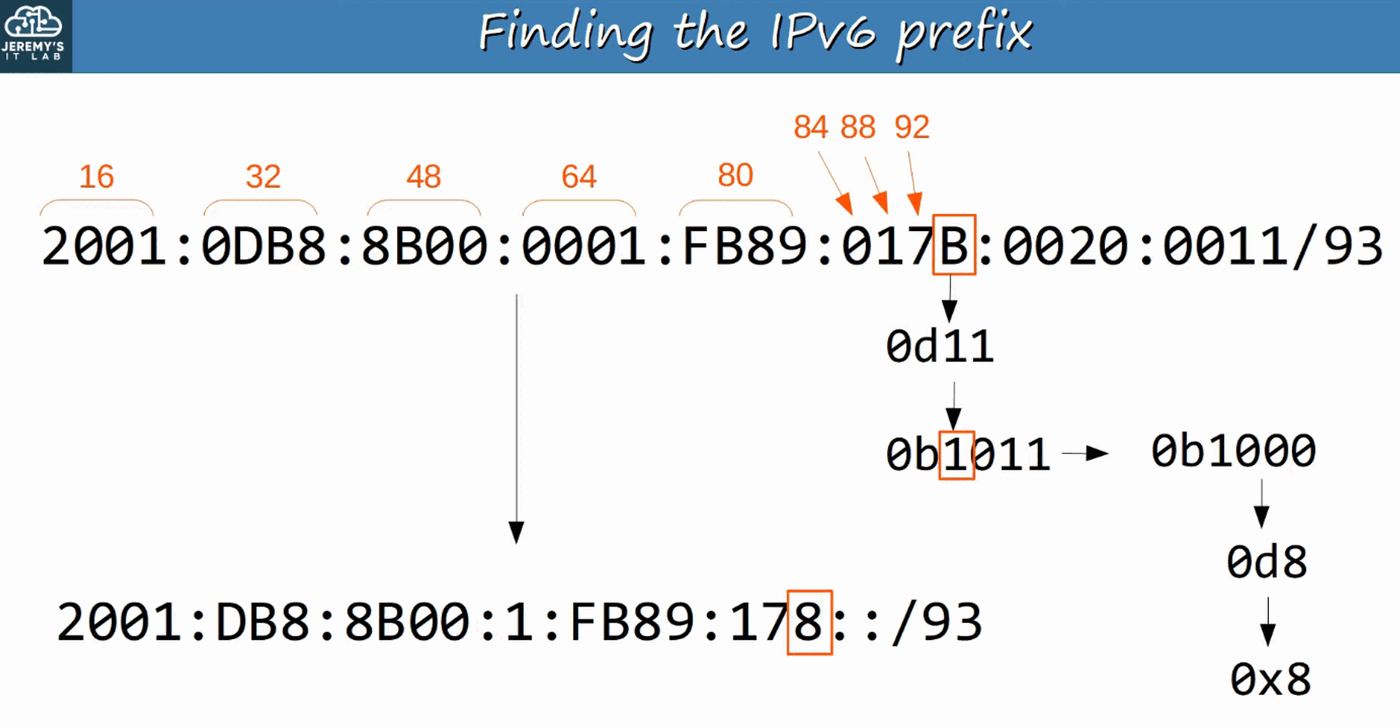
\includegraphics[keepaspectratio,alt={image}]{images/32-ipv6-part1/img-015.png}}
\end{figure}

\begin{figure}
\centering
\pandocbounded{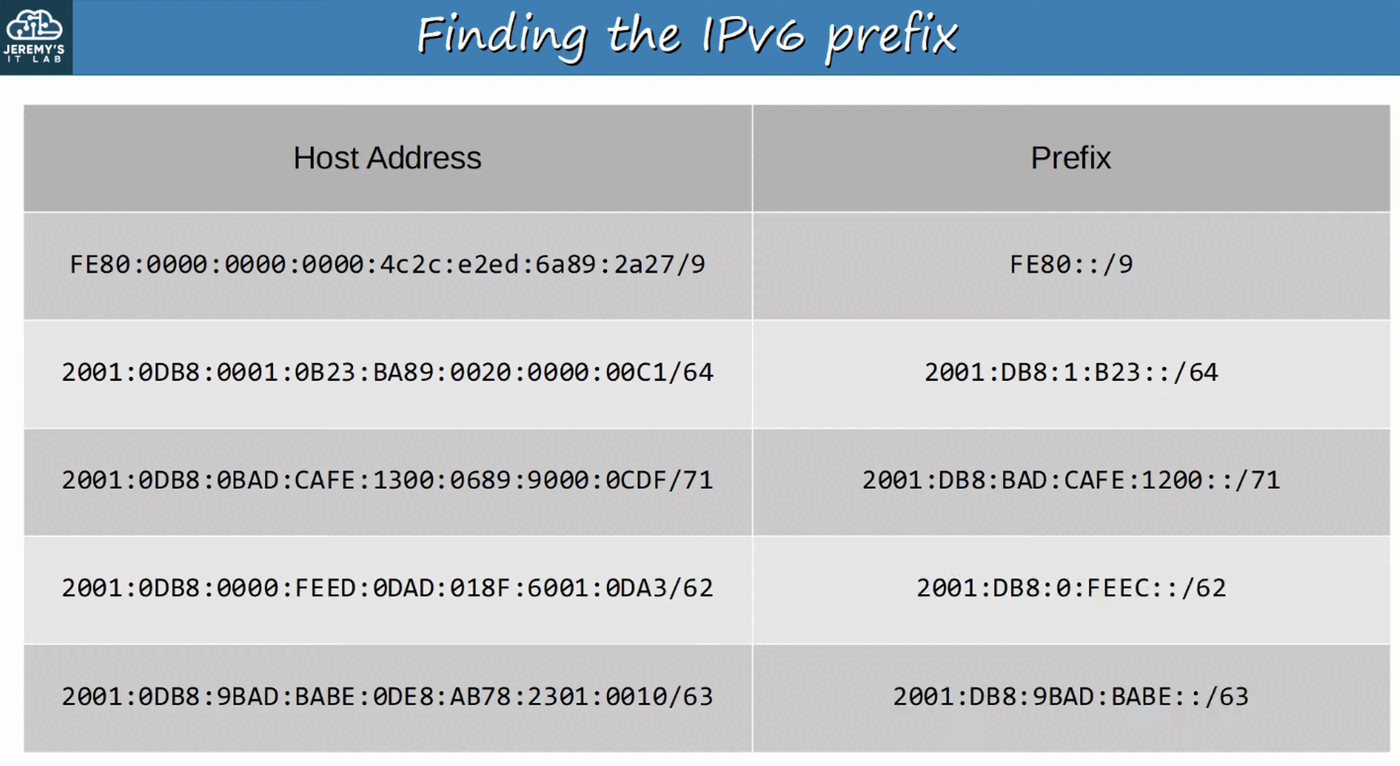
\includegraphics[keepaspectratio,alt={image}]{images/32-ipv6-part1/img-016.png}}
\end{figure}

CONFIGURING IPv6 ADDRESSES

\begin{figure}
\centering
\pandocbounded{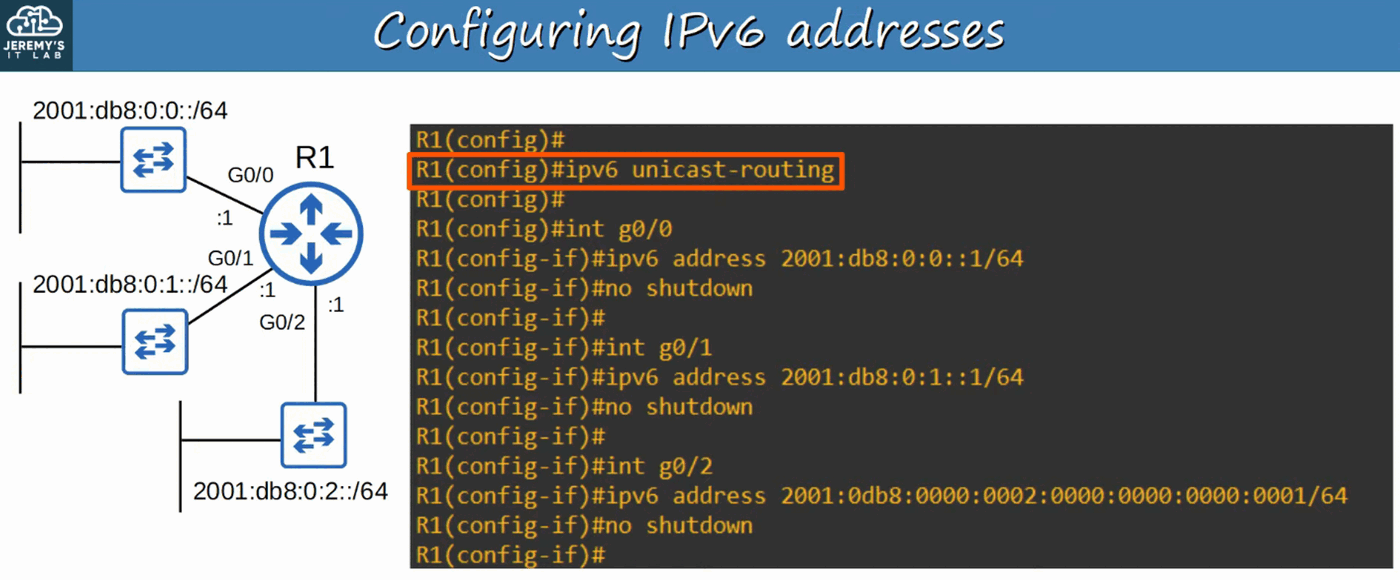
\includegraphics[keepaspectratio,alt={image}]{images/32-ipv6-part1/img-017.png}}
\end{figure}

This allows the ROUTER to perform IPv6 ROUTING

\begin{tipbox}

R1(config) \#ipv6 unicast-routing

\end{tipbox}

Configuring an INTERFACE with an IPv6 Address

\begin{tipbox}

R1(config) \#int g0/0 R1(config-if) \#ipv6 address 2001:db8:0:0::1/64
R1(config) \#no shutdown

\end{tipbox}

You can also type out the full address (if necessary)

\begin{figure}
\centering
\pandocbounded{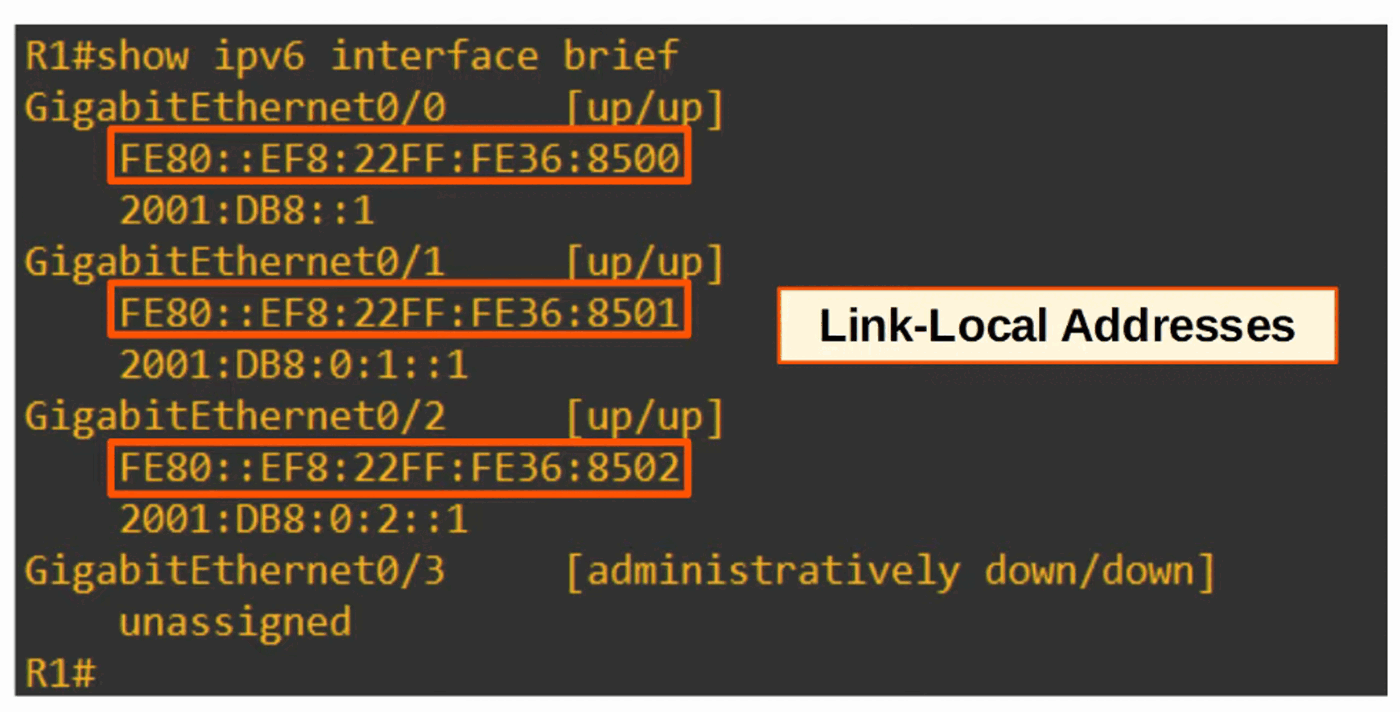
\includegraphics[keepaspectratio,alt={image}]{images/32-ipv6-part1/img-018.png}}
\end{figure}

NOTE ABBREVIATED IPv6 ADDRESSES SHOWN

LINK-LOCAL ADDRESSES are automatically added when creating an IPv6
INTERFACE (Covered in IPv6 - PART 2 Lecture)
